\chapter{Fundamentos teóricos}

%\section{Control clásico}


%Una vez conseguida una estimación del estado en el instante $t$ ,  $S_t$ se necesita emplear un algoritmo de control que genere	las acciones $A_t$ correspondientes para llegar al estado $S_{t'}$ deseado de forma óptima.

%\tb{BUCLE DE CONTROL}


%Existe una gran cantidad de controladores clásicos que se pueden emplear para generar estos comandos, por ejemplo: PID o LQR.
%En este trabajo se han explorado 2 controladores: el primero de ellos se trata de un controlador clásico PID y el segundo consiste en un controlador no lineal modelizado por una red neuronal.

\section{Controlador PID}




Un regulador PID es un controlador lineal realimentado. Matemáticamente se expresa como 
\begin{equation}
	u(t) = \overbrace{\raisebox{0ex}[2.2\height]{$K_p e(t)$}}^\text{P} +\overbrace{K_i \int_{0}^{t}e(\tau)d\tau}^\text{I} + \overbrace{ K_d \frac{de(t)}{dt}}^\text{D}\;
\end{equation}

donde $e(t)$ es la señal de control, $u(t)$ representa la salida del regulador y $K_p,K_i,K_d$ son parámetros ajustables de los cuales depende la dinámica y la estabilidad del sistema. Como se puede observar, el regulador consta de tres partes: la parte proporcional (P) tiene en cuenta el error actual, la parte integral (I) tiene en cuenta el histórico de los errores y la parte derivativa (D) tiene en cuenta la estimación del error futuro.
\section{Redes neuronales artificiales} 
 Una red neuronal artificial (ANN) esta compuesta por un conjunto de nodos o perceptrones interconectados entre sí. Estos perceptrones se agrupan en capas ``ocultas'', se les atribuye este nombre debido a que todos los nodos de una capa se interconectan con todos los nodos de la capa anterior, por lo que después del aprendizaje de la red no se sabe cuales son los perceptrones de la capa anterior que influyen en un nodo.
 
 
 
 \begin{figure}[htb!]
 	\centering
 	\begin{tikzpicture}[]
 	\def\nodedist{35pt}
 	\def\layerdist{80pt}
 	\def\pindist{20pt}
 	
 	\tikzstyle{every pin edge}=[signal]
 	\tikzstyle{annot} = [text width=4em, text centered]
 	
 	\foreach \y in {1,...,3}
 	\node[inputnode, pin={[pin edge={latex-}, pin distance=\pindist]left:Entrada \y: $x_\y$}] 
 	(I\y) at (0,-\y*\nodedist) {$a_\y^{[0]}$};  
 	
 	\foreach \y in {1,...,4}
 	\node[hiddennode] 
 	(H\y) at ($(\layerdist,-\y*\nodedist) +(0, 0.5*\nodedist)$) {$a_\y^{[1]}$};
 	
 	\foreach \y in {1,...,1}
 	\node[outputnode, pin={[pin edge={-latex}, pin distance=\pindist]right:\Large$\hat y$}]
 	(O\y) at ($(I2) + (2*\layerdist, 0)$) {$a_\y^{[2]}$};
 	
 	\foreach \dest in {1,...,4}
 	\foreach \source in {1,...,3}
 	\draw[signal] (I\source) -- (H\dest);
 	
 	\foreach \dest in {1,...,1}
 	\foreach \source in {1,...,4}
 	\draw[signal] (H\source) edge (O\dest);
 	
 	\node[annot, above=4pt of H1] (hl) {Capa oculta};
 	\node[annot] at (I1 |- hl) {Capa de entrada};
 	\node[annot] at (O1 |- hl) {Capa de salida};
 	\end{tikzpicture}
 	\caption{Esquema de una red neuronal artificial}
 \end{figure}
 

Cada perceptron es la unidad mínima de computación de una ANN, estas unidades se dividen en dos partes, una parte lineal y una parte de activación o no lineal. En la parte lineal o parte ``Z'' se computa una regresión lineal de las salidas de los nodos anteriores.
 \begin{align}
 	z^{[l]}_i &= \sum_{j=0}^{n^{[l-1]}} {w_{ij}\cdot a^{[l-1]}_j} + b_i  \qquad &i=0,..,n^{[l]} \\
 	a^{[l]}_i &= g\left(z^{[l]}_i\right) \qquad  &i=0,..,n^{[l]}
 \end{align}
 El superíndice $[l]$ hace referencia a la capa en la que se encuentra el elemento. Siendo $n^{[l]}$ el número de nodos de la capa $l$-ésima.
 
 
 A los coeficientes $w_{ij}$ se les denomina los pesos del perceptrón y $b_i$ es el término independiente de la regresión. 
 
 
 \begin{figure}[htb!]
 	
 	\centering
 	\begin{tikzpicture}[
 	% define styles    
 	init/.style={ 
 		draw, 
 		circle, 
 		inner sep=2pt,
 		font=\Huge,
 		join = by -latex
 	},
 	squa/.style={ 
 		font=\Large,
 		join = by -latex
 	}
 	]
 	% Top chain x1 to w1
 	\begin{scope}[start chain=1]
 	\node[on chain=1] at (0,1.5cm)  (x1) {$a_1^{[l-1]}$};
 	\node[on chain=1,,label=above:\parbox{1cm}{pesos},join=by o-latex] (w1) {$w_1$};
 	\end{scope}
 	% Middle chain x2 to output
 	\begin{scope}[start chain=2]
 	\node[on chain=2] (x2) {$a_2^{[l-1]}$};
 	\node[on chain=2,join=by o-latex] {$w_2$};
 	\node[on chain=2,init] (sigma) {$\displaystyle\Sigma$};
 	\node[on chain=2,squa,label=above:{\parbox{2cm}{\centering Regresión lineal}}]   {$z_i^{[l]}$};
 	\node[on chain=2,squa,label=above:{\parbox{2cm}{\centering Función de\\ activacion}}]   {$a_i^{[l]}= g(z_i^{[l]})$};
 	\node[on chain=2,squa,label=above:Salida,join=by -latex] {$y_{out}$};
 	\end{scope}
 	% Bottom chain x3 to w3
 	\begin{scope}[start chain=3]
 	\node[on chain=3] at (0,-1.5cm) 
 	(x3) {$a_3^{[l-1]}$};
 	\node[on chain=3,join=by o-latex]
 	(w3) {$w_3$};
 	\end{scope}
 	% Bias
 	\node[label=above:\parbox{2cm}{\centering \text{$\;$} \\ $b$}] at (sigma|-w1) (b) {};
 	% Arrows joining w1, w3 and b to sigma
 	\draw[-latex] (w1) -- (sigma);
 	\draw[-latex] (w3) -- (sigma);
 	\draw[o-latex] (b) -- (sigma);
 	% left hand side brace
 	\draw[decorate,decoration={brace,mirror}] (x1.north west) -- node[left=10pt] {Entrada} (x3.south west);
 	
 	\end{tikzpicture}
 	\caption{Esquema de un perceptrón}
 	\label{esquema_perceptron}
 	
 \end{figure}
 
 La función $g(z)$ es la función de activación del nodo. Estas funciones proporcionan no linealidad a la red neuronal, permitiendo a estas la capacidad de generar modelos con grandes no linealidades. Las funciones de activación más frecuentes en la literatura son:
 
 \begin{itemize}
 	\item Función sigmoide: 
 	\begin{equation}
 	\sigma(z) = \frac{1}{1+e^{-z}} \qquad\qquad \sigma(z):\mathbb{R} \rightarrow [0,1]
 	\end{equation}
	\begin{figure}[htb!]
		\centering
		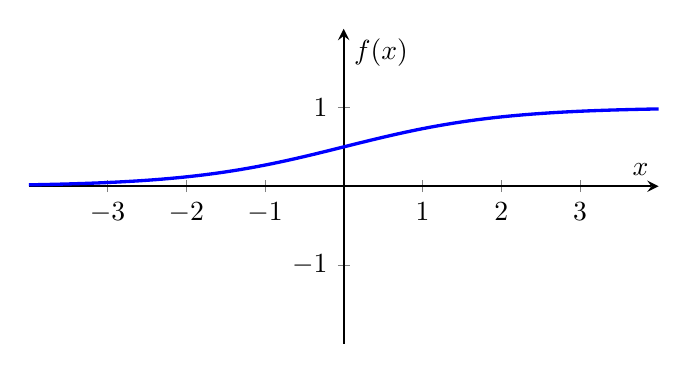
\begin{tikzpicture}[]
		\begin{axis}[ 
		%title=$\tanh(x)$,
		axis x line=middle, xmin=-4, xmax=4, xtick={-3,...,3}, xlabel=$x$,
		axis y line=middle, ymin=-2, ymax=2, ytick={-1,...,1}, ylabel=$f(x)$,
		legend pos=north west,
		legend style={empty legend, draw=none},
		scale only axis=true,
		width=8cm, height=4cm,
		thick,
		samples=101] 
		\addplot[blue, very thick] {1/(1+exp(-x))};
		%\addlegendentry{$\tanh(x)$}
		\end{axis}
		\end{tikzpicture}
		\caption{Función sigmoide}
	\end{figure}

	\item Tangente hiperbólica: 
	\begin{equation}
	\tanh(z) = \frac{e^z-e^{-z}}{e^z+e^{-z}} \qquad\qquad \tanh(z):\mathbb{R} \rightarrow [-1,1]
	\end{equation}
	
	\begin{figure}[htb!]
		\centering
		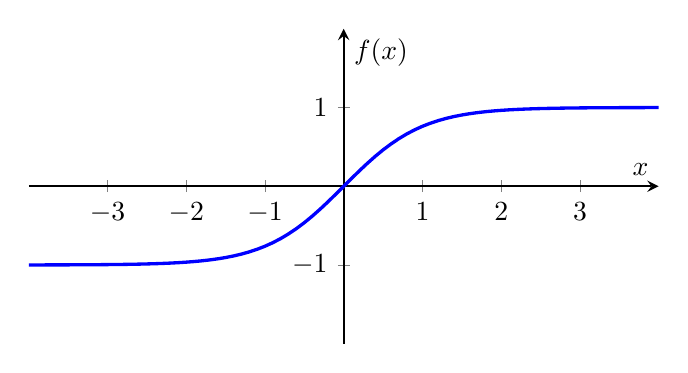
\begin{tikzpicture}[]
		\begin{axis}[ 
		%title=$\tanh(x)$,
		axis x line=middle, xmin=-4, xmax=4, xtick={-3,...,3}, xlabel=$x$,
		axis y line=middle, ymin=-2, ymax=2, ytick={-1,...,1}, ylabel=$f(x)$,
		legend pos=north west,
		legend style={empty legend, draw=none},
		scale only axis=true,
		width=8cm, height=4cm,
		thick,
		samples=101] 
		\addplot[blue, very thick] {tanh(x))};
		%\addlegendentry{$\tanh(x)$}
		\end{axis}
		\end{tikzpicture}
		
		\caption{Función tangente hiperbólica}
	\end{figure}

	\item ReLu (del inglés \textit{Rectified Linear Unit}): 
	
	\begin{equation}
		g(z) = \text{max}(0,z) \qquad\qquad g(z):\mathbb{R} \rightarrow [0,+\infty]
	\end{equation}
\\
	\begin{figure}[htb!]
		\centering
		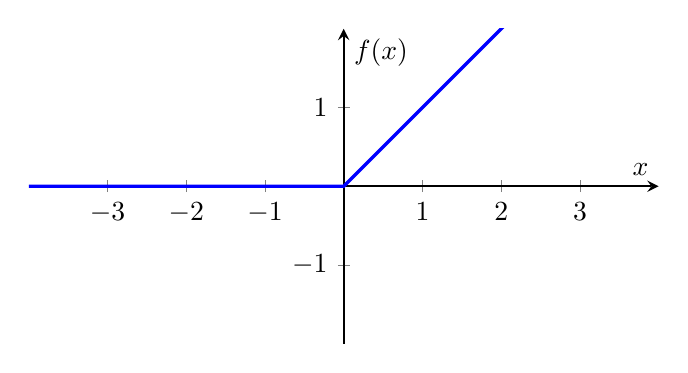
\begin{tikzpicture}[]
		\begin{axis}[ 
		%title=$\tanh(x)$,
		axis x line=middle, xmin=-4, xmax=4, xtick={-3,...,3}, xlabel=$x$,
		axis y line=middle, ymin=-2, ymax=2, ytick={-1,...,1}, ylabel=$f(x)$,
		legend pos=north west,
		legend style={empty legend, draw=none},
		scale only axis=true,
		width=8cm, height=4cm,
		thick,
		samples=101] 
		\addplot[blue, very thick] {(\x < 0) * (0) + (\x > 0) * (\x)};
		%\addlegendentry{$\tanh(x)$}
		\end{axis}
		\end{tikzpicture}
		\caption{Función ReLu}
	\end{figure}
	

\end{itemize} 
  
 Para conseguir que la red neuronal realice predicciones precisas es necesario ajustar los pesos de la red, a este proceso es al que se denomina entrenamiento o aprendizaje. En el paradigma del aprendizaje supervisado este entrenamiento se realiza sometiendo a la red a ejemplos cuya salida es conocida. El objetivo de la red es minimizar el error de la esperanza de la estimación con respecto a la salida real del ejemplo. Formalmente, se define una función de coste $\mathcal{J}$ la cúal se quiere minimizar. Por ejemplo, una función de coste típica para problemas de clasificación binaria es la \textit{binary cross-entropy}:
 
 \begin{align}
 \mathcal{L}(\hat{y},y)&=-\big(y\log\hat{y} + (1-y)\log(1-\hat{y})\big)\\ 
 \mathcal{J}(w,b)&=\frac{1}{m}\sum_{i=1}^{m}{\mathcal{L}\big(\hat{y}^{(i)},{y}^{(i)}\big)}
 \end{align}
 donde $\hat{y}$ denota la estimación de la salida realizada por parte de la red, $y$ la salida conocida y $m$ el número de ejemplos. 
 
 Para minimizar esta función de coste, que depende de los pesos de la red, existen distintos métodos, uno de los más usados es el método del descenso de gradiente. Este método emplea la ``propagación hacia atrás'' (del inglés \textit{back propagation}) de la red neuronal, esto consiste en obtener las derivadas parciales de la función de coste con respecto a los pesos de cada nodo y actualizar estos pesos en la dirección opuesta al máximo gradiente.
 
 \begin{align}
 	w:= w - \alpha\; &\frac{\partial\mathcal{J}(w,b)}{\partial w}\\
 	b:= b - \alpha\; &\frac{\partial\mathcal{J}(w,b)}{\partial b}
 \end{align}
 
 donde $\alpha$ denota la tasa de aprendizaje, es decir, lo rápido que varian estos pesos.

 



\section{Aprendizaje por refuerzo}

El aprendizaje por refuerzo o \textit{Reinforcement learning} \cite{sutton2018reinforcement} es un área del aprendizaje automático o \textit{Machine Learning} en el que un agente interactúa con un entorno buscando la mejor acción a realizar en función de su estado actual.


\begin{figure}[htb!]
	\centering
	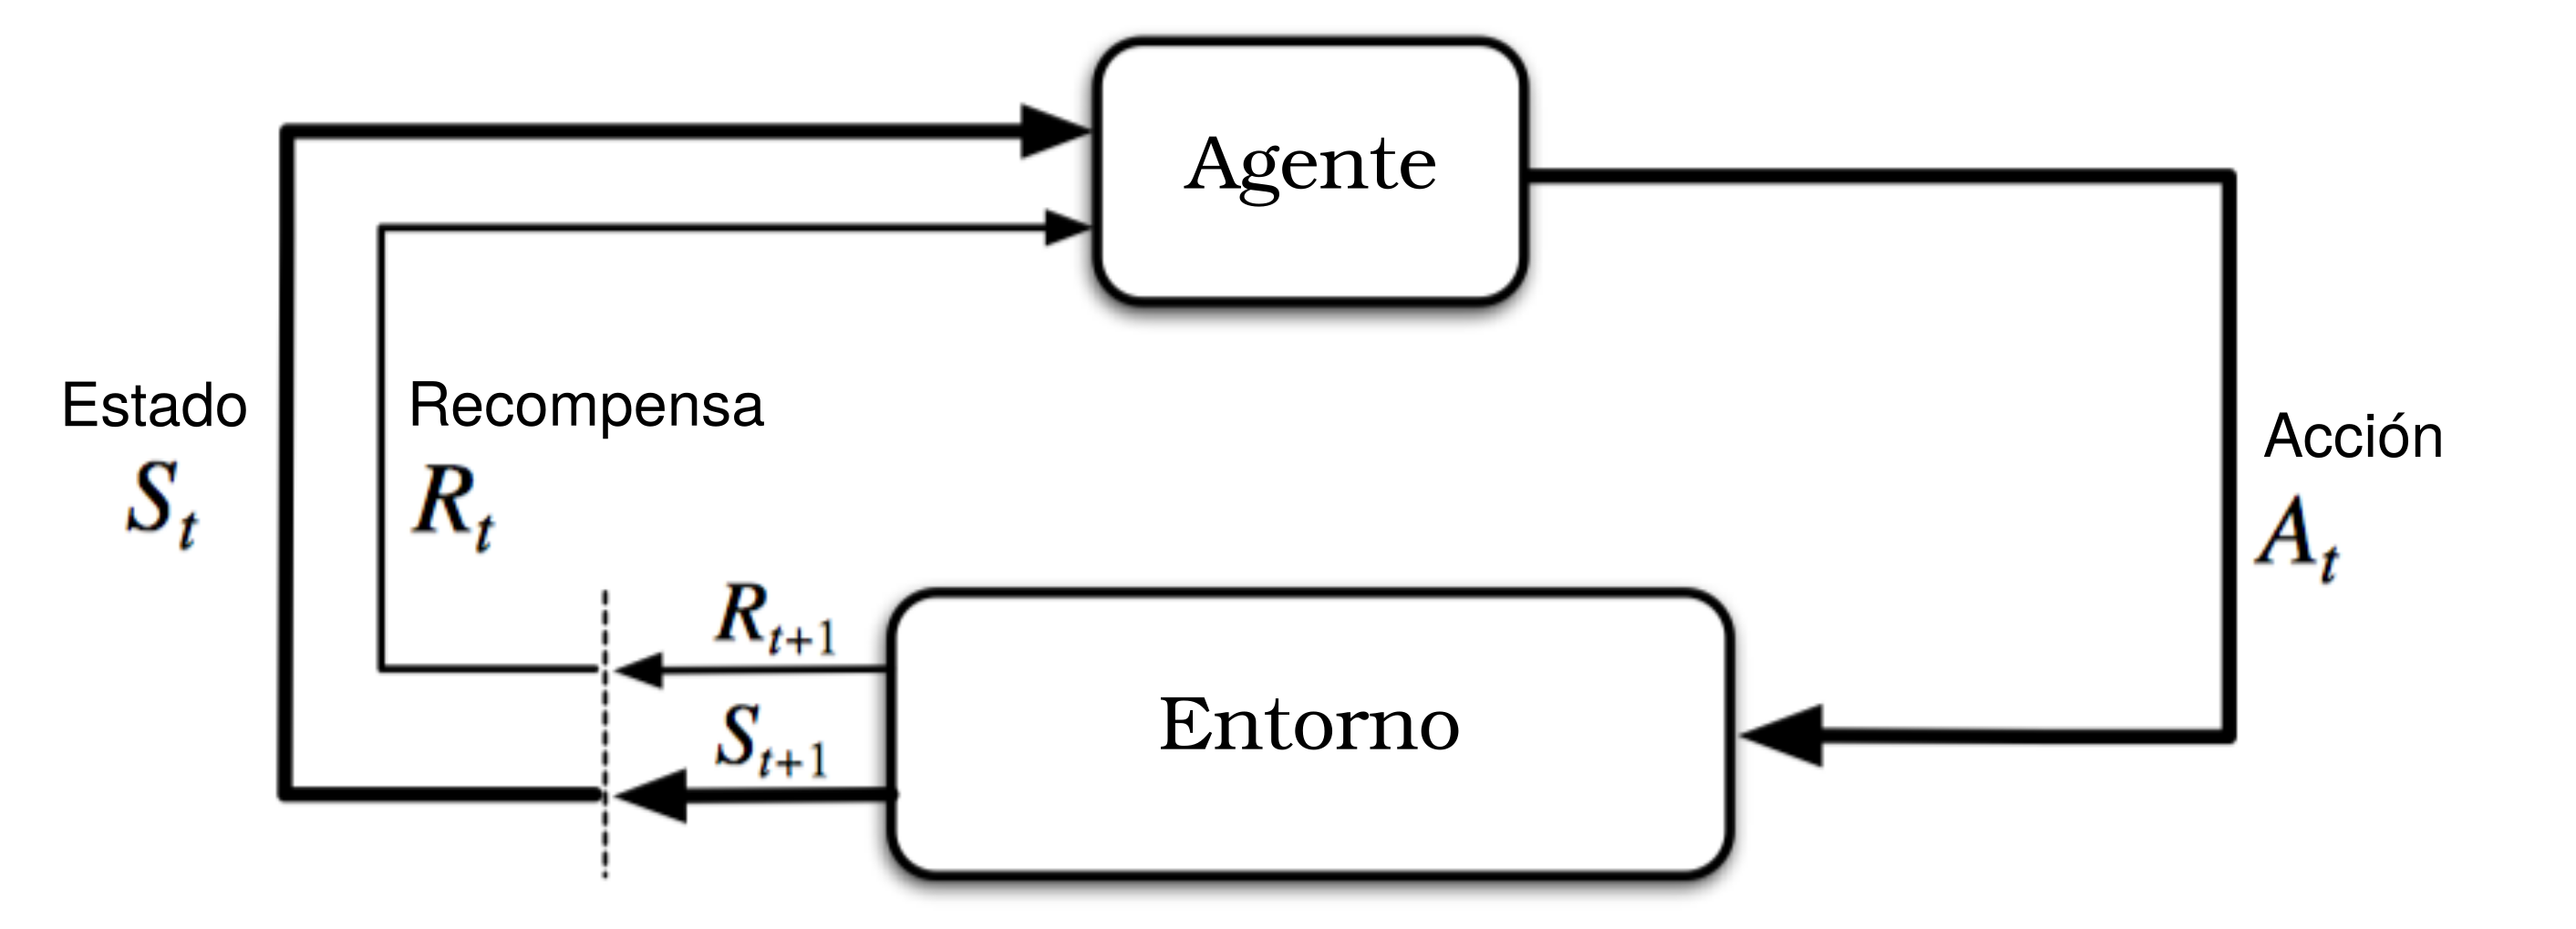
\includegraphics[width=0.8\textwidth]{background/RL_diagram}
	\caption{Diagrama canónico del bucle de interacción entorno-agente}
	\label{hardware:droneImg}
\end{figure}


Se diferencia de otras técnicas de aprendizaje automático es su enfoque orientado a la interacción directa con el entorno, sin basarse en un modelo completo del entorno o en un conjunto de ejemplos supervisados.

\subsubsection{Elementos del aprendizaje por refuerzo}
Además del agente y el entorno se pueden identificar tres elementos principales más en un sistema de aprendizaje con refuerzo:

\begin{itemize}
	\item[$\bullet$] \textbf{Política ($\pi$)}  (Proveniente del termino anglosajón \textit{policy}, el cual es el término empleado en el estado del arte). Define el conjunto de acciones que debe realizar el agente para conseguir maximizar su recompensa en función su estado, el cuál es percibido a través del entorno. La \textit{policy} constituye el núcleo del agente y nos permite determinar su comportamiento. Estas políticas pueden ser estocásticas.
	
	\item[$\bullet$] \textbf{Recompensa} ($Rt$). 
	Define el objetivo del agente en un problema de aprendizaje por refuerzo. En cada salto de tiempo (\textit{step}) el agente recibe una recompensa por parte del entorno (un número). 
	
	\item[$\bullet$] \textbf{Función de valor} ($V^\pi_s$). Representa la máxima recompensa que puede esperar obtener un agente desde un estado concreto, empleando una política concreta, es decir, tiene en cuenta la recompensa a largo plazo, no solo la inmediata.
	\begin{equation}
		V^\pi(s)= \mathbb{E}_\pi\left[\sum_{k=0}^{\infty}{\gamma^k r_{t+k+1}}\Big|s_t=s\right]
	\end{equation}
		
\end{itemize}
Algunos algoritmos de aprendizaje por refuerzo requieren de la definición de un \textbf{modelo del entorno}. Este modelo permite predecir el comportamiento que va a tener el entorno a lo largo del tiempo.

\subsubsection{Procesos de decisión de Markov}

El aprendizaje por refuerzo emplea el marco formal de los procesos de decisión de Markov (\textit{MDP}) en los cuales para definir la interacción entre en agente y el entorno en términos de estados, acciones y recompensas.

Un proceso de decisión de Markov está compuesto por la 4-tupla $(S,A,P_a,R_a)$ donde:

\begin{itemize}
	\item \textbf{S} representa el estado del agente.
	\item \textbf{A} es el conjunto de acciones que puede realizar el agente. $A_s$ denota las acciones que puede realizar el agente desde un estado $s$.
	\item \textbf{$\boldsymbol{P_a(s,s')}$} = $Pr\big(s_{t+1} = s' \;|\; s_t = s , a_t = a  \big)$. Partiendo de un estado $s$, $P_a$ representa la probabilidad de pasar al estado $s'$ tomando la acción $a$.
	\item \textbf{$\boldsymbol{R_a(s,s')}$} denota la recompensa inmediata que recibiría el agente al realizar la transicion de $s$ a $s'$ mediante la acción $a$.
\end{itemize}

Estos procesos cumplen la propiedad de Markov, es decir, que el pasado no influye en el agente, lo único relevante es el estado actual.

El problema principal de los MDP es encontrar la secuencia de acciones que debe realizar el agente para maximizar la recompensa a largo plazo, es decir, encontrar la política $\pi$ 
óptima, que permita maximizar la recompensa. Una vez encontrada la política $\pi$ óptima el problema se reduce a una cadena de Markov, dado que la acción $a$ a realizar en un estado $s$ viene completamente definida por el estado $s$ y la probabilidad $P_a$. 

La política $\pi$ óptima es aquella que maximice la recompensa acumulada, es decir, la suma decontada de las recompensas instantáneas percibidas por el entorno:

\begin{equation}
	G_t = R_{t+1} + \gamma R_{t+2} + \gamma^2 R_{t+3} + ... = \sum_{k=0}^{\infty}\gamma^k R_{
	t+k+1}
\end{equation}

donde $\gamma$ es el factor de descuento, el cual debe cumplir $0 \le \gamma \le 1$, cuanto mayor sea este factor menos importante es la recompensa inmediata. 

En este trabajo se han trabajado con 2 tipos de algoritmos de aprendizaje por refuerzo: métodos basados en \textit{Q-learning} y métodos de gradiente de las políticas.

\subsection{Algoritmos de \textit{Q-learning}}
Los algoritmos de Q-learning se basan en la función estado-acción, también conocida como función Q, de ahí el nombre de estos algoritmos. Esta función denota el valor de tomar una acción en un estado siguiendo una política $\pi$. Formalmente, la función Q se define como

\begin{equation}
	Q^\pi(s,a) =  \mathbb{E}_\pi\left[\sum_{k=0}^{\infty}{\gamma^k r_{t+k+1}}\Big|s_t=s,a_t = a\right]
\end{equation}

La diferencia entre la función Q y la función de valor radica en que la función de valor cuantifica lo ``bueno'' que es un estado concreto, mientras que la función Q evalúa la conveniencia de tomar una acción concreta en un estado determinado. Este matiz se empleará posteriormente para definir la función de ventaja en el apartado \ref{ALG_GRAD_POL}.

El objetivo de estos algoritmos se basa en obtener la función óptima $Q^*$, esta función cumple la ecuación de Bellman 
	\begin{equation}
		Q^*(s,a)= \mathbb{E}_{s'}\left[r+\gamma\;\underset{a'}{\text{max}}\; Q^*(s',a')\big|s,a\right]
	\end{equation}
siendo s'y a' la secuencia siguiente de estados y acciones, respectivamente.

Basándose en esta ecuación la función $Q^*$ se podría calcular como un proceso iterativo de la forma
	\begin{equation}
	Q_{i+1}(s,a)= \mathbb{E}\left[r+\gamma\;\underset{a'}{\text{max}}\; Q_i(s',a')\big|s,a\right]
	\end{equation}

Aunque este proceso converge a la funcion estado-acción óptima, $Q_i \rightarrow Q^*$ cuando $i \rightarrow \infty$ \cite{sutton2018reinforcement}, esto no es práctico, debido a que esta aproximación de la función Q se estima de forma independiente para cada secuencia concreta, sin generalizar. En lugar de esto, se suele emplear una función que se aproxime a esta función estado-acción. En los casos en los que esta función sea aproximada por una red neuronal, ésta se denota por $Q(s,a; \theta)$ siendo $\theta$ los pesos de esta red-Q (\textit{Q-network}). 

La función de pérdida que se intenta minimizar para entrenar esta red es
\begin{equation}\label{eq:1}
	L_i(\theta_i) = \mathbb{E}_{s,a\sim\rho(s,a)}\left[\left(y_i - Q(s,a;\theta_i)\right)^2\right]
\end{equation} 
donde $y_i= \mathbb{E}_{s'}[ r + \gamma \; {\text{max}_{a'}} \; Q(s',a';\theta_{i-1})]$ es el objetivo(\textit{target}) para la iteración i y $\rho(s,a)$ es la distribución del comportamiento, es decir, distribución de probabilidad de las secuencias $a', s'$ a lo largo del tiempo.

Esta función de pérdida se puede minimizar con algoritmos de optimización como el Descenso de gradientes estocástico (SDG).

\subsubsection{DQN}

El algoritmo DQN (\textit{Deep Q-network}) es un algoritmo basado en \textit{Q-learning} desarrollado por Mnih et al. \tb{citar} en 2015. Con este algoritmo la empresa DeepMind consiguió desarrollar un agente capaz de jugar a los juegos de la clásica consola Atari, superando con creces el rendimiento de los jugadores profesionales en algunos juegos. Este algoritmo está diseñado para actuar sobre un conjunto de acciones discretas, como son las acciones de la consola Atari.

El nombre del algoritmo, hace referencia al empleo de una red neuronal profunda (\textit{Deep Network}) como aproximador de la función Q (\textit{Q-network}).
Este algoritmo introduce, principalmente, dos modificaciones sobre los algoritmos Q que favorecen el aprendizaje:

\begin{enumerate}
	\item \textbf{Creación de un ``contenedor de repeticiones''} (\textit{buffer replay}) en el que se almacenan las experiencias del agente en cada iteración temporal $e_t=(s_t,a_t,r_t,s_{t+1})$ en un conjunto de datos $D_t=\{e_1,...,e_t\}$ recabados durante varios episodios.
	
	Este contenedor se emplea para obtener una muestra de aleatoria de experiencias y constituir un pequeño lote con el que optimizar la red-Q.
	
	Emplear este método proporciona proporciona varias ventajas notorias:
	
	\begin{itemize}
		\item Permite el empleo de los datos recabados en cada paso temporal para optimizar los pesos en múltiples interacciones, lo que se traduce en un mejor aprovechamiento de las experiencias del agente.
		
		\item Al tomar muestras de forma consecutiva el aprendizaje se vuelve ineficiente debido a la alta correlación entre las muestras. Al tomar muestras aleatorias del contenedor se consigue romper esta correlación.
	\end{itemize}
	
	\item \textbf{Empleo de una red objetivo }$Q'$ para la actualización de pesos.  Cada $C$ actualizaciones se clona la red $Q$ para obtener la red objetivo $\hat Q$. Esta red objetivo $\hat Q$ es la que emplea para realizar el cómputo de la expresión $y_i$ durante la actualización de pesos.
	\begin{equation}
	y_i= \mathbb{E}_{s'}[ r + \gamma \; {\text{max}_{a'}} \; \hat Q(s',a';\theta^-)]
	\end{equation}
	En este algoritmo se realiza la optimización mediante el algoritmo SDG de la funcion de pérdida \ref{eq:1}.  Cada $C$ pasos se reinicia la función Q con los valores del objetivo $Q=\hat Q$.
	
	Al emplear una red con parámetros desactualizados, a la hora de actualizar la red, se  reduce las oscilaciones en el entrenamiento y se favorece la convergencia.
	
\end{enumerate}

\subsubsection{DDPG}

El algoritmo DDPG (\textit{Deep Deterministic Policy Gradient}), creado por Lillicrap et al. \tb{citar} en 2016, adapta las ideas del DQN a un dominio de acciones continuo. Este algoritmo emplea la filosofía actor-crítico, en la que una parte evalúa la bondad de una accion en un estado (crítico) y  otra define la política que debe realizar el agente (actor).

La función actor $\mu(s|\theta^\mu)$ devuelve la acción que se debe realizar en el estado $s$, es decir, la política $\pi$ que debe seguir el agente. El crítico $Q(s,a)$ se entrena empleando la identidad de Bellman al igual que en los algoritmos de aprendizaje-Q.

Para actualizar los pesos de la función actor se emplea el gradiente de la función de coste empleados por Silver et al. \tb{citar DPG paper} 

	\begin{align}
		\nabla_{\theta^\mu}J &\approx \mathbb{E}_{s_t \sim \rho}\left[ \nabla_{\theta^\mu} Q(s,a |\theta^Q)|_{s=s_t,a=\mu(s_t|\theta^\mu)}\right]\\
		&=  \mathbb{E}_{s_t \sim \rho}\left[ \nabla_{a} Q(s,a |\theta^Q)|_{s=s_t,a=\mu(s_t)} \nabla_{\theta^\mu}\; \mu(s|\theta^\mu)|_{s=s_t}    \right]\nonumber 
	\end{align}

Para favorecer la exploración del algoritmo se genera una política de exploración $\mu'$ se le añade ruido $\mathcal{N}$ a la política del actor
	\begin{equation}
		 \mu'(s_t)=\mu(s_t|\theta^\mu_t) + \mathcal{N}
	\end{equation}

este ruido se puede generar de varias formas, en el artículo se emplea ruido generado mediante el proceso de Ornstein-Uhlenbeck \tb{(citar)} para generar ruido correlado temporalmente.

Este algoritmo mantiene el contenedor de repeticiones y el empleo de redes objetivo del DQN aunque añade alguna modificación en esta última. En vez de reiniciar el valor de la red $R$ con el valor de la red objetivo $\hat R$ cada $C$ épocas, en el DDPG, esta actualización de las redes $Q$ y $\mu$ se realiza de forma suave mediante una media ponderada móvil (\textit{Weighted Moving Average})

\begin{align}
\theta ^{\hat Q} &\leftarrow \tau \theta ^ Q + (1 - \tau)\theta^{\hat Q}\\
\theta ^{\hat \mu} &\leftarrow \tau \theta ^ \mu + (1 - \tau)\theta^{\hat \mu}
\end{align}
con $\tau \ll  1$. De esta forma los pesos de la red cambian de forma suave, lo que favorece la estabilidad del entrenamiento. 

\subsection{Algoritmos de gradiente de políticas} \label{ALG_GRAD_POL}

\subsubsection{TRPO}
\subsubsection{PPO}